In de Computer Management applicatie vind je onder Storage een kopje Disk Management. Daar kunnen we informatie opvragen over onze disks.

\begin{minipage}[t]{\linewidth}
\raggedright
\adjustbox{valign=t}{%
   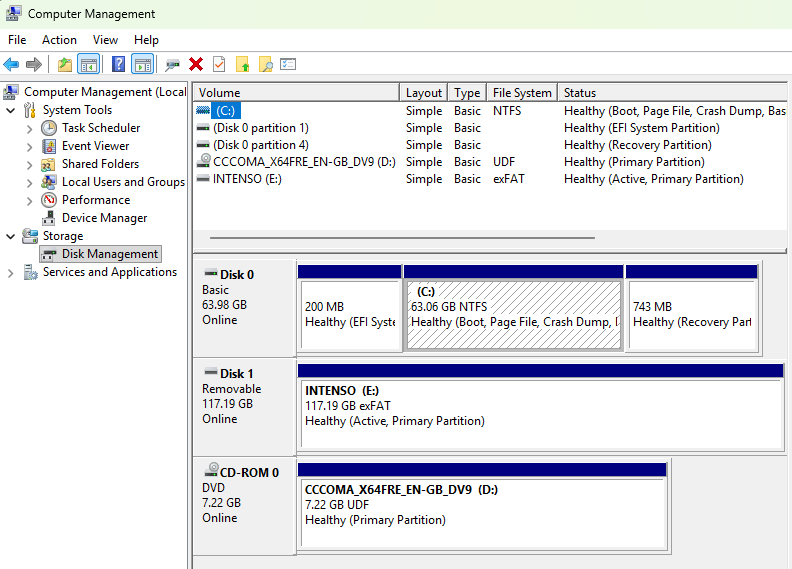
\includegraphics[width=0.99\linewidth]{computer_management-disks.png}%
}
\end{minipage}

We zien in het plaatje een harddisk (Disk 0), een USB-stick (Disk 1) en een DVD (CD-ROM 0). We zien tevens dat ze allemaal gebruik maken van een ander filesystem. De partitie op de harddisk die onze C: drive is gebruikt NTFS, de USB-stick exFAT en de DVD UDF.
\begin{description}
\item[UDF] Universal Disk Format: Een bestandssysteem dat veel gebruikt wordt voor media die \'e\'en keer geschreven worden en daarna alleen gelezen. Je komt dit tegen op data CD's en DVD's. UDF is een extensie en de opvolger van ISO-9960. Als we praten over een ISO-image dan bedoelen we tegenwoordig vaak UDF.
\item[exFAT] extensible File Allocation Table: is de opvolger van FAT het bestandssysteem dat door Microsoft gebruikt wordt sinds DOS. exFAT ontwikkeld door Microsoft en is simpel en open source. Er is ondersteuning voor exFAT in Windows, Linux en MacOS X, daarmee is het het ideale bestandssysteem om data uit te wisselen tussen verschillende systemen. Je komt het dan ook vaak tegen op USB-sticks.
\item[NTFS] New Technology File System: Een door Microsoft ontwikkeld bestandssysteem dat gebruikt wordt vanaf Windows NT. Het is een relatief complex bestandssysteem dat veel extra data (META-data) kan bijhouden. Die metadata bestaat voornamelijk uit wie welke rechten heeft op de bestanden en directories.
\end{description}

In het Volume overzicht zien we onze C: drive. Gebruiken we de rechermuisklik op deze drive dan krijgen we een menutje waaruit we Properties kunnen selecten. Properties bestaat uit verschillende tabs:
\begin{description}
\item[General] geeft een overzicht van het gebruik van de disk. Een klik op details brengt je naar Settings, System Storage, Show more categories.
\item[Hardware] Geeft je meer specieke informatie over een drive, via deze ingang kan je ook driver updates doen voor een drive.
\item[Security] Hierin kan je zetten wie er welke rechten heeft op de partitie.
\item[Sharing] Hier kan je je disk delen met andere gebruikers of systemen op het netwerk.
\item[Quota] Hier kan je quota zetten. Dit is standaard gedisabled. Via het knopje \textquote{Quota Entries} kan je per gebruiker aangeven hoeveel diskspace deze mag gebruiken. Dat is de quota per gebruiker.
\item[Previous Versions] is een overzicht van oude restore points
\item[Tools] Bevat de tools Error checking en Optimise and defragmentation drive. Deze onderdelen worden in volgende secties behandeld.
\end{description}

